\documentclass[12pt]{article}
\usepackage[margin=1in]{geometry}
\setlength{\parindent}{0pt}
\setlength{\parskip}{5pt}
%\pagenumbering{gobble}% 

\usepackage{amsmath,amsthm,amssymb}
\usepackage{graphicx}
\usepackage{bm}
\usepackage{float}
\newtheorem{euclidtheorem}{Proposition}[section]
\newtheorem{classtheorem}{Theorem}
\newtheorem{theorem}{Theorem}[section]
\newtheorem{challenge}[theorem]{Challenge}
\newtheorem{question}[theorem]{Question}
\newtheorem{problem}[theorem]{Problem}

\newtheorem{theorempiece}{Theorem}[theorem]
\newtheorem{classtheorempiece}{Theorem}[classtheorem]
\newtheorem{challengepiece}{Challenge}[theorem]
\newtheorem{questionpiece}{Question}[theorem]
\newtheorem{problempiece}{Problem}[theorem]

\renewcommand*{\theeuclidtheorem}{\Roman{section}.\arabic{theorem}}
\renewcommand*{\thetheorem}{\arabic{section}.\arabic{theorem}}
\renewcommand*{\theclasstheorem}{\Alph{theorem}}
\renewcommand*{\thechallenge}{\arabic{section}.\arabic{theorem}}
\renewcommand*{\thequestion}{\arabic{section}.\arabic{theorem}}
\renewcommand*{\theproblem}{\arabic{section}.\arabic{theorem}}
\renewcommand*{\thetheorempiece}{\arabic{section}.\arabic{theorem}.\alph{theorempiece}}
\renewcommand*{\thechallengepiece}{\arabic{section}.\arabic{theorem}.\alph{challengepiece}}
\renewcommand*{\thequestionpiece}{\arabic{section}.\arabic{theorem}.\alph{questionpiece}}
\renewcommand*{\theproblempiece}{\arabic{section}.\arabic{theorem}.\alph{problempiece}}

\usepackage{tikz}
\usetikzlibrary{arrows,shapes,decorations,automata,backgrounds,petri}
\usepackage[latin1]{inputenc}
\usepackage{verbatim}
\usepackage{wasysym} 
\usepackage{setspace}

\title{Homework 1 of Statistical Machine Learning}
\author{Wang Yikai, 2017310740}
\date{\today}

\begin{document}

\maketitle

{\Large \bf 1 Mathematics Basics}
\par
\bigskip
{\large \bf 1.1 Optimization}
\par
Use the Lagrange multiplier method to solve the following problem:
\begin{align*}
\min_{x_1,x_2}&\;x_1^2+x_2^2=1\\
s.t.\;&x_1+x_2-1=0\\
&x_1-2x_2\geq0
\end{align*}
The Lagrange function is:
$$L(x_1,x_2,\alpha,\beta)=x_1^2+x_2^2+\alpha(2x_2-x_1)+\beta(x_1+x_2-1)$$
where $\alpha$ and $\beta$ are Lagrange multipliers.
\par
The dual problem is:
\begin{align*}
&\max_{\alpha,\beta}\min_{x_1,x_2}\;L(x_1,x_2,\alpha,\beta)\\
&\,s.t.\;\alpha\geq0
\end{align*}
First find the derivatives of $L(x_1,x_2,\alpha,\beta)$ w.r.t. $x_1,x_2$, and let the derivatives equal to zero:
\begin{align*}
&\frac{\partial L(x_1,x_2,\alpha,\beta)}{\partial x_1}=2x_1-\alpha+\beta=0\,\Rightarrow\,x_1=\frac{\alpha-\beta}{2}\\
&\frac{\partial L(x_1,x_2,\alpha,\beta)}{\partial x_2}=2x_2+2\alpha+\beta=0\,\Rightarrow\,x_2=-\alpha-\frac{\beta}{2}
\end{align*}
Therefore the dual problem turns to:
\begin{align*}
&\max_{\alpha,\beta}\;g(\alpha,\beta)=-\frac{5}{4}\alpha^2-\frac{1}{2}\beta^2-\frac{1}{2}\alpha\beta-\beta\\
&\,s.t.\;\alpha\geq0
\end{align*}
Compute the derivatives of $g(\alpha,\beta)$ w.r.t. $\alpha,\beta$, there are:
\begin{align*}
&\frac{\partial g(\alpha,\beta)}{\partial \alpha}=-\frac{5}{2}\alpha-\frac{1}{2}\beta=0\\
&\frac{\partial g(\alpha,\beta)}{\partial \beta}=-\beta-\frac{1}{2}\alpha-1=0\\
&\Rightarrow\, \alpha=\frac{2}{9},\,\beta=-\frac{10}{9}
\end{align*}
Therefore the optimal value of the dual problem is:
$$\max_{\alpha,\beta}\min_{x_1,x_2}\;L(x_1,x_2,\alpha,\beta)=-\frac{4}{9}$$
The optimal solution is:
$$x_1=\frac{2}{3},\;x_2=\frac{1}{3}$$

\bigskip
{\large \bf 1.2 Calculus}
\par
(1) Prove the recursion formula of Gamma function:
\begin{align*}
\Gamma(x+1)&=\int_{0}^{\infty}u^{x-1}e^{-u}du\\
&=-\int_{0}^{\infty}u^{x-1}de^{-u}\\
&=\left.-u^x e^{-u}\right|_0^\infty+\int_{0}^{\infty}x u^{x-1}e^{-u}du\\
&=\lim_{u\rightarrow\infty}-u^x e^{-u}+x\int_{0}^{\infty}u^{x-1}e^{-u}du\\
&=x\int_{0}^{\infty}u^{x-1}e^{-u}du\\
&=x\Gamma(x)
\end{align*}
(2) Prove the relationship between gamma function and beta function:
\begin{align*}
\Gamma(a)\Gamma(b)&=\int_{u=0}^{\infty}e^{-u}u^{a-1}du\int_{v=0}^{\infty}e^{-v}v^{b-1}dv\\
&=\int_{v=0}^{\infty}\int_{u=0}^{\infty}e^{-u-v}u^{a-1}v^{b-1}dudv
\end{align*}
Changing variables by $u=f(z,\mu)=z\mu$ and $v=g(z,\mu)=z(1-\mu)$, and let $|J(z,\mu)|$ be the absolute value of the Jacobian determinant of $u=f(z,\mu)$ and $v=g(z,\mu)$:
\begin{align*}
\Gamma(a)\Gamma(b)&=\int_{z=0}^{\infty}\int_{\mu=0}^{1}e^{-z}(z\mu)^{a-1}[z(1-\mu)]^{b-1}|J(z,\mu)|d\mu dz\\
&=\int_{z=0}^{\infty}\int_{\mu=0}^{1}e^{-z}(z\mu)^{a-1}[z(1-\mu)]^{b-1}z d\mu dz\\
&=\int_{z=0}^{\infty}e^{-z}(z\mu)^{a-1}z^{a+b-1}dz\int_{\mu=0}^{1}\mu^{a-1}(1-\mu)^{b-1}d\mu\\
&=\Gamma(a+b)\int_{\mu=0}^{1}\mu^{a-1}(1-\mu)^{b-1}d\mu
\end{align*}
Therefore there is:
$$\mathrm{Beta}(a,b)=\int_{0}^{1}\mu^{a-1}(1-\mu)^{b-1}d\mu=\frac{\Gamma(a)\Gamma(b)}{\Gamma(a+b)}$$
This result implies that the Beta distribution is normalized.

\bigskip
{\large \bf 1.3 Probability}
\par
The prior distribution $p(\lambda;\alpha,\beta)$ follows Gamma distribution:
$$p(\lambda;\alpha,\beta)=\frac{\beta^\alpha}{\Gamma(\alpha)}\lambda^{\alpha-1}e^{-\beta\lambda}$$
The likelihood function $p(x|\lambda)$ follows Poisson distribution:
$$p(x|\lambda)=\frac{\lambda^x}{x!}e^{-\lambda}$$
Then the posterior distribution is:
\begin{align*}
p(\lambda|x)&=\frac{p(x|\lambda)\,p(\lambda;\alpha,\beta)}{p(x)}\\
&=\frac{\beta^\alpha\lambda^{\alpha+x-1}e^{-(\beta+1)\lambda}}{\Gamma(\alpha)\,x!\,p(x)}\\
&\propto \lambda^{\alpha+x-1}e^{-(\beta+1)\lambda}
\end{align*}
Therefore the posterior distribution $p(\lambda|x)$ follows Gamma distribution $\Gamma(\lambda|\alpha+x,\beta+1)$, which implies that the Gamma distribution can serve as a conjugate prior to the Poisson distribution.

\bigskip
{\large \bf 1.4 Stochastic Process}
\par

We need to observe a consecutive pattern which has the length of $k+1$, one $H$ and $k$ $T$.
\par 
Consider establishing a Markov process: the initial state means currently the coins are all $T$; there are $k+1$ middle states, and the $i$th middle state means currently we have $i$ coins that match the pattern; at last we have one final state, means that we have observed the given pattern. Obviously in this Markov process, the initial state and $k+1$ middle states are $\bm{\mathrm{non-recurrent\;states}}$, and the final state is an $\bm{\mathrm{absorption\;state}}$. In non-recurrent states, if we get another coin that matches the next term of the pattern, the state will change to the next state, otherwise the state will return to the initial state, and the two situations have equal probability. The diagram of this Markov process is shown as below, where all the probability of transitions in the diagram are 0.5:

\begin{center}
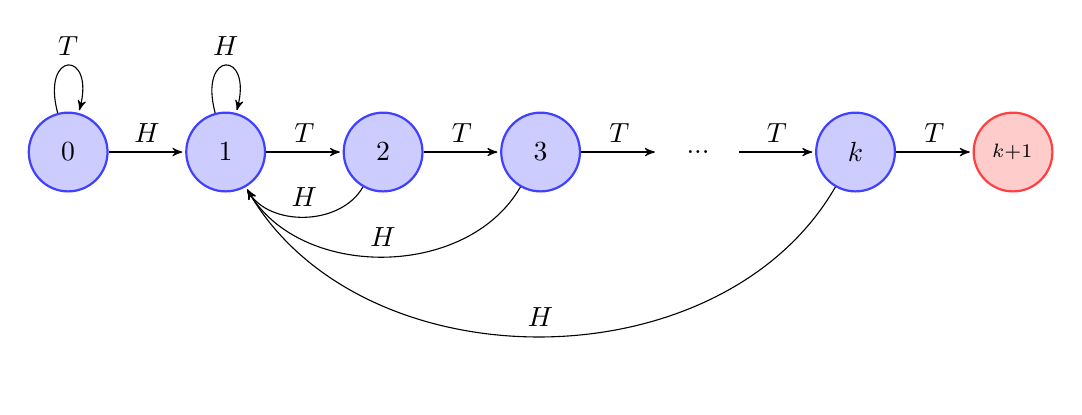
\begin{tikzpicture}[node distance=2cm,>=stealth',bend angle=60,auto]

% 	\draw[black,|-|] (2.7,0.9) -- (8.5,0.9);
%     \draw[black,-] (5.6,0.9) -- (5.6,0.9)
%         node[above] {$k$};

    \tikzstyle{start}=[circle,thick,draw=blue!75,fill=blue!20,minimum size=10mm]
    \tikzstyle{transition}=[circle,thick,draw=blue!75,fill=blue!20,minimum size=10mm]
    \tikzstyle{slh}=[circle,thick,minimum size=10mm]
    \tikzstyle{absorption}=[circle,thick,draw=red!75,fill=red!20,minimum size=10mm]
    \begin{scope}
		\node [start] (i) {$0$}
            edge [loop above] node [above] {$T$} (i);
        \node [transition] (c1) [right of=i]{$1$}
        	edge [loop above] node [above] {$H$} (c1)
            edge [pre] node [above] {$H$} (i);
        \node [transition] (c2)  [right of=c1] {$2$}
            edge [pre] node [above] {$T$} (c1)
            edge [post, bend left] node [above] {$H$} (c1);
        \node [transition] (c3) [right of=c2] {$3$}
            edge [pre] node [above] {$T$} (c2)
            edge [post, bend left] node [above] {$H$} (c1);
        \node [slh] (sl) [right of=c3] {$...$}
            edge [pre] node [above] {$T$} (c3);
        \node [transition] (c4) [right of=sl]{$k$}
            edge [pre] node [above] {$T$} (sl)
            edge [post, bend left] node [above] {$H$} (c1);
        \node [absorption] (c5) [right of=c4]{$_{k+1}$}
            edge [pre] node [above] {$T$} (c4);
  	\end{scope}
%   \begin{pgfonlayer}{background}
%     \filldraw [line width=4mm,join=round,black!10]
%       (c5.north  -| c5.east)  rectangle (c1.south  -| c1.west);
%   \end{pgfonlayer}
\end{tikzpicture}
\end{center}
The question turns to calculate the expectation time from a non-recurrent state to the absorption state.
The transition matrix with $(k+2)\times(k+2)$ dimensions is:
\begin{equation*}
\bm{P}=\left[ \begin{array}{cccccccc}
0.5 & 0.5 & 0 & 0 & 0 & \cdots & 0 & 0\\
0 & 0.5 & 0.5 & 0 & 0 & \cdots & 0 & 0\\
0 & 0.5 & 0 & 0.5 & 0 & \cdots & 0 & 0\\
0 & 0.5 & 0  & 0 & 0.5 & \cdots & 0 & 0\\
\vdots & \vdots & \vdots & \vdots & \vdots & \ddots & \vdots & \vdots\\
0 & 0.5 & 0  & 0 & 0 & \cdots & 0.5 & 0\\
0 & 0.5 & 0  & 0 & 0 & \cdots & 0 & 0.5\\
0 & 0 & 0  & 0 & 0 & \cdots & 0 & 1
\end{array} 
\right]_{(k+2)\times(k+2)}
\end{equation*}
Suppose $\bm{D}$ equals to the first $(k+1)\times(k+1)$ dimensions of $\bm{P}$:
\begin{equation*}
\bm{D}=\left[ \begin{array}{ccccccc}
0.5 & 0.5 & 0 & 0 & 0 & \cdots & 0\\
0 & 0.5 & 0.5 & 0 & 0 & \cdots & 0\\
0 & 0.5 & 0 & 0.5 & 0 & \cdots & 0\\
0 & 0.5 & 0  & 0 & 0.5 & \cdots & 0\\
\vdots & \vdots & \vdots & \vdots & \vdots & \ddots & \vdots \\
0 & 0.5 & 0  & 0 & 0 & \cdots & 0.5\\
0 & 0.5 & 0  & 0 & 0 & \cdots & 0
\end{array} 
\right]_{(k+1)\times(k+1)}
\end{equation*}
Let $\bm{g}=[1,1,...,1]^T$, which has $(k+1)$ dimensions, and $\bm{I}$ is a unit matrix with $(k+1)\times(k+1)$ dimensions. The expected number of total tosses equals to the first number of the vector $(\bm{I}-\bm{D})^{-1}\bm{g}$. Let $\bm{Q}=\bm{I}-\bm{D}$, there is:
\begin{equation*}
\bm{Q}=\left[ \begin{array}{ccccccc}
0.5 & -0.5 & 0 & 0 & 0 & \cdots & 0\\
0 & 0.5 & -0.5 & 0 & 0 & \cdots & 0\\
0 & -0.5 & 1 & -0.5 & 0 & \cdots & 0\\
0 & -0.5 & 0  & 1 & -0.5 & \cdots & 0\\
\vdots & \vdots & \vdots & \vdots & \vdots & \ddots & \vdots \\
0 & -0.5 & 0  & 0 & 0 & \cdots & -0.5\\
0 & -0.5 & 0  & 0 & 0 & \cdots & 1
\end{array} 
\right]_{(k+1)\times(k+1)}
\end{equation*}
Therefore:
\begin{align*}
(\bm{I}-\bm{D})^{-1}\bm{g}&=\bm{Q}^{-1}\bm{g}=\frac{\bm{Q}^*}{\mathrm{det}\left(\bm{Q}\right)}\bm{g}=2^{k+1}\bm{Q}^*\bm{g}
\end{align*}
in this equation $\bm{Q}^*=\left(\bm{Q}_{ij}\right)_{(k+1)\times(k+1)}$, and $\bm{Q}_{ij}=(-1)^{i+j}\bm{M}_{ij}$, where $\bm{M}_{ij}$ is the determinant of $\bm{Q}$ when deleting the $i$th row and the $j$th column. Then the first number of $2^{k+1}\bm{Q}^*\bm{g}$ is the expectation time, which is found to be $2^{k+1}$.
\par
Or there is another easier way to get the result. Suppose $t(i)$ is the expected time from the state $i$ to the absorption state $k+1$. Suppose $p_{ij}$ is the transition probability from state $i$ to $j$, and the specific value can be obtained by the matrix $P$ shown before. There is:
$$t(i)=1+\sum_{j\in\{j:i\rightarrow j\}}p_{i,j}t(j)$$
Given that $t(k+1)=0$, we can get $t(0)=2^{k+1}$.

\bigskip
\bigskip
{\Large \bf 2 SVM}
\bigskip
\par
Consider the regression problem with training data $\{(\bm{x}_i, y_i)\}_{i=1}^N$ where $\bm{x}_i\in\mathbb{R}^d,y_i\in\mathbb{R}$. The primal problem of linear SVM is:
\begin{align*}
&\min_{\bm{\omega},b,\bm{\xi},\hat{\bm{\xi}}}\frac{1}{2}\|\bm{\omega}\|^2+C\sum_{i=1}^N\left(\xi_i+\hat{\xi}_i\right)\\
&\;s.t.\;y_i\leq\bm{\omega}^T\bm{x}_i+b+\epsilon+\xi_i,\;1\leq i \leq N \\
&\quad\quad y_i\geq\bm{\omega}^T\bm{x}_i+b-\epsilon-\hat{\xi}_i,\;1\leq i \leq N \\
&\quad\quad\xi_i\geq 0,\;1\leq i \leq N\\
&\quad\quad\hat{\xi}_i\geq 0,\;1\leq i \leq N 
\end{align*}
where $C$ is a constant and $\epsilon>0$ denotes a fixed small value.
\par
The corresponding Lagrangian of SVM is:
\begin{align*}
L(\bm{\omega},b,\bm{\xi},\hat{\bm{\xi}},\bm{\alpha},\hat{\bm{\alpha}},\bm{\beta},\hat{\bm{\beta}})&=\frac{1}{2}\|\bm{\omega}\|^2+C\sum_{i=1}^N\left(\xi_i+\hat{\xi}_i\right)+\sum_{i=1}^N\alpha_i\left[y_i-\left(\bm{\omega}^T\bm{x}_i+b+\epsilon+\xi_i\right)\right]\\
&-\sum_{i=1}^N\hat{\alpha}_i\left[y_i-\left(\bm{\omega}^T\bm{x}_i+b-\epsilon-\hat{\xi}_i\right)\right]-\sum_{i=1}^N\beta_i\xi_i-\sum_{i=1}^N\hat{\beta}_i\hat{\xi}_i\\
&=\frac{1}{2}\bm{\omega}^T\bm{\omega}+C\left(\bm{\xi}+\hat{\bm{\xi}}\right)^T\bm{1}+\sum_{i=1}^N\alpha_i\left[y_i-\left(\bm{\omega}^T\bm{x}_i+b+\epsilon+\xi_i\right)\right]\\
&-\sum_{i=1}^N\hat{\alpha}_i\left[y_i-\left(\bm{\omega}^T\bm{x}_i+b-\epsilon-\hat{\xi}_i\right)\right]-\bm{\xi}^T\bm{\beta}-\hat{\bm{\xi}}^T\hat{\bm{\beta}}
\end{align*}
where $\bm{\alpha}\geq\bm{0},\,\hat{\bm{\alpha}}\geq\bm{0},\,\bm{\beta}\geq\bm{0},\,\hat{\bm{\beta}}\geq\bm{0}$ are Lagrange multipliers.

\par
The dual Lagrangian problem of SVM is:
$$\max_{\bm{\alpha},\hat{\bm{\alpha}},\bm{\beta},\hat{\bm{\beta}}}\,\min_{\bm{\omega},b,\bm{\xi},\hat{\bm{\xi}}}\,L(\bm{\omega},b,\bm{\xi},\hat{\bm{\xi}},\bm{\alpha},\hat{\bm{\alpha}},\bm{\beta},\hat{\bm{\beta}})$$

To solve the dual Lagrangian problem, the dual function of SVM needs to be derived first:
$$g(\bm{\alpha},\hat{\bm{\alpha}},\bm{\beta},\hat{\bm{\beta}})=\min_{\bm{\omega},b,\bm{\xi},\hat{\bm{\xi}}}\,L(\bm{\omega},b,\bm{\xi},\hat{\bm{\xi}},\bm{\alpha},\hat{\bm{\alpha}},\bm{\beta},\hat{\bm{\beta}})$$

Let the derivatives of $L$ w.r.t. $\bm{\omega},\,b,\bm{\xi},\hat{\bm{\xi}}$ equal to zero:
\begin{align*}
&\left.\frac{\partial L}{\partial \bm{\omega}}\right|_{\bm{\omega}^*}=\bm{\omega}^*-\sum_{i=1}^N\left(\alpha_i-\hat{\alpha}_i\right)\bm{x}_i=0\;\Rightarrow\;\bm{\omega}^*=\sum_{i=1}^N\left(\alpha_i-\hat{\alpha}_i\right)\bm{x}_i\\
&\left.\frac{\partial L}{\partial b}\right|_{b^*}=0\;\Rightarrow\;\sum_{i=1}^N\left(\alpha_i-\hat{\alpha}_i\right)=0\\
&\left.\frac{\partial L}{\partial \bm{\xi}}\right|_{\bm{\xi}^*}=C\bm{1}-(\bm{\alpha}+\bm{\beta})=0\;\Rightarrow\;
\left\{
\begin{array}{lr}
\bm{\beta}=C\bm{1}-\bm{\alpha}\\
0\leq\bm{\alpha}\leq C\bm{1}
\end{array}
\right.\\
&\left.\frac{\partial L}{\partial \hat{\bm{\xi}}}\right|_{\hat{\bm{\xi}}^*}=C\bm{1}-(\hat{\bm{\alpha}}+\hat{\bm{\beta}})=0\;\Rightarrow\; 
\left\{
\begin{array}{lr}
\hat{\bm{\beta}}=C\bm{1}-\hat{\bm{\alpha}}\\
0\leq\hat{\bm{\alpha}}\leq C\bm{1}
\end{array}
\right.
\end{align*}

So the dual function is:
\begin{align*}
g(\bm{\alpha},\hat{\bm{\alpha}},\bm{\beta},\hat{\bm{\beta}})&=L(\bm{\omega}^*,b^*,\bm{\xi}^*,\hat{\bm{\xi}}^*,\bm{\alpha},\hat{\bm{\alpha}},\bm{\beta},\hat{\bm{\beta}})\\
&=\frac{1}{2}\|\bm{\omega}^*\|^2+\sum_{i=1}^N\left(\alpha_i-\hat{\alpha_i}\right)\left[y_i-\left({\bm{\omega}^*}^T\bm{x}_i+b^*\right)\right]+\epsilon\left(\bm{\alpha}+\hat{\bm{\alpha}}\right)^T\bm{1}\\
&=\frac{1}{2}\|\bm{\omega}^*\|^2+\sum_{i=1}^N\left(\alpha_i-\hat{\alpha_i}\right)\left(y_i-{\bm{\omega}^*}^T\bm{x}_i\right)+\epsilon\left(\bm{\alpha}+\hat{\bm{\alpha}}\right)^T\bm{1}\\
&=\frac{1}{2}\left\|\sum_{i=1}^N\left(\alpha_i-\hat{\alpha}_i\right)\bm{x}_i\right\|^2+\sum_{i=1}^N\left(\alpha_i-\hat{\alpha_i}\right)\left\{y_i-\left[\sum_{j=1}^N\left(\alpha_j-\hat{\alpha}_j\right)\bm{x}_j\right]^T\bm{x}_j\right\}+\epsilon\left(\bm{\alpha}+\hat{\bm{\alpha}}\right)^T\bm{1}\\
&=\epsilon\left(\bm{\alpha}+\hat{\bm{\alpha}}\right)^T\bm{1}+\left(\bm{\alpha}-\hat{\bm{\alpha}}\right)^T\bm{y}-\frac{1}{2}\left\|\sum_{i=1}^N\left(\alpha_i-\hat{\alpha}_i\right)\bm{x}_i\right\|^2\\
&=\epsilon\left(\bm{\alpha}+\hat{\bm{\alpha}}\right)^T\bm{1}+\left(\bm{\alpha}-\hat{\bm{\alpha}}\right)^T\bm{y}-\frac{1}{2}\left(\bm{\alpha}-\hat{\bm{\alpha}}\right)^T\bm{G}\left(\bm{\alpha}-\hat{\bm{\alpha}}\right)
\end{align*}
where $\bm{G}\in\mathbb{R}^{N\times N},\,G_{ij}=\bm{x}_i^T\bm{x}_j.$

\par
Therefore the dual problem turns to:
\begin{align*}
&\max_{\bm{\alpha},\hat{\bm{\alpha}}}\,\epsilon\left(\bm{\alpha}+\hat{\bm{\alpha}}\right)^T\bm{1}+\left(\bm{\alpha}-\hat{\bm{\alpha}}\right)^T\bm{y}-\frac{1}{2}\left(\bm{\alpha}-\hat{\bm{\alpha}}\right)^T\bm{G}\left(\bm{\alpha}-\hat{\bm{\alpha}}\right)\\
&\,s.t.\;0\leq\bm{\alpha}\leq C\bm{1},\,0\leq\hat{\bm{\alpha}}\leq C\bm{1},\,\left(\bm{\alpha}-\hat{\bm{\alpha}}\right)^T\bm{1}=0
\end{align*}
where the definitions and constrains of $\bm{G}$ is shown before.

\bigskip
\bigskip
{\Large \bf 3 IRLS for Logistic Regression}
\par
\bigskip
For a binary classification problem $\{(x_i,y_i)\}_{i=1}^N\;(x_i\in\mathbb{R}^d,\,y_i\in\{0,1\})$, the probabilistic decision rule according to logistic regression is:
$$P_{\bm{\omega}}\left(y|\bm{x}\right)=\frac{\mathrm{exp}\left(y\bm{\omega}^T\bm{x}\right)}{1+\mathrm{exp}\left(\bm{\omega}^T\bm{x}\right)}$$
And hence the log-likelihood is:
\begin{align*}
\mathcal{L}\left(\bm{\omega}\right)&=\mathrm{log}\prod_{i=1}^N P_{\bm{\omega}}\left(y_i|\bm{x}_i\right)\\
&=\sum_{i=1}^N\left\{y_i\bm{\omega}^T\bm{x}_i-\mathrm{log}\left[1+\mathrm{exp}\left(\bm{\omega}^T\bm{x}_i\right)\right]\right\}
\end{align*}
The gradient of $\mathcal{L}\left(\bm{\omega}\right)$ w.r.t. $\bm{\omega}$ is:
\begin{align*}
\bm{g}&=\frac{\partial\mathcal{L}\left(\bm{\omega}\right)}{\partial\bm{\omega}}\\
&=\sum_{i=1}^N\left[y_i\bm{x}_i-\frac{\mathrm{exp}\left(\bm{\omega}^T\bm{x}_i\right)\bm{x}_i}{1+\mathrm{exp}\left(\bm{\omega}^T\bm{x}_i\right)}\right]\\
&=\sum_{i=1}^N\left[y_i-\sigma\left(\bm{\omega}^T\bm{x}_i\right)\right]\bm{x}_i\\
&=\bm{X}\left(\bm{y}-\bm{\mu}\right)
\end{align*}
where $\sigma(a)=\frac{\mathrm{exp}(a)}{1+\mathrm{exp}(a)}$ is the sigmoid function and there is $\frac{d\sigma}{da}=\sigma(1-\sigma)$; $\bm{X}=[\bm{x}_1,\bm{x}_2,...,\bm{x}_N]_{d\times N}$, $\mu_i=\sigma\left(\bm{\omega}^T\bm{x}_i\right)$.
\par
The Hessian matrix of $\mathcal{L}\left(\bm{\omega}\right)$ is:
\begin{align*}
\bm{H}&=\frac{\partial^2\mathcal{L}\left(\bm{\omega}\right)}{\partial\bm{\omega}\partial\bm{\omega}^T}\\
&=\frac{\partial\left[\bm{\bm{X}\left(\bm{y}-\bm{\mu}\right)}\right]}{\partial \bm{\omega}^T}\\
&=-\bm{X}\mathrm{diag}\left\{\mu_i\left(1-\mu_i\right)\bm{x}_i^T\right\}\\
&=-\bm{X}\bm{R}\bm{X}^T
\end{align*}
where $R_{ii}=\mu_i\left(1-\mu_i\right)=\sigma\left(\bm{\omega}^T\bm{x}_i\right)\left[1-\sigma\left(\bm{\omega}^T\bm{x}_i\right)\right]$.
\par
In least square estimate of linear regression, we have:
$$\bm{\omega}=\left(\bm{X}\bm{X}^T\right)^{-1}\bm{X}\bm{y}$$
In IRLS, we have:
\begin{align*}
\bm{\omega}_{t+1}&=\bm{\omega}_t-\bm{H}^{-1}\bm{g}\\
&=\bm{\omega}_t+\left(\bm{X}\bm{R}\bm{X}^T\right)^{-1}\bm{X}\left(\bm{y}-\bm{\mu}\right)\\
&=\left(\bm{X}\bm{R}\bm{X}^T\right)^{-1}\left[\bm{X}\bm{R}\bm{X}^T\bm{\omega}_t+\bm{X}\left(\bm{y}-\bm{\mu}\right)\right]\\
&=\left(\bm{X}\bm{R}\bm{X}^T\right)^{-1}\bm{X}\bm{R}\bm{z}
\end{align*}
where $\bm{z}=\bm{X}^T\bm{\omega}_t+\bm{R}^{-1}\left(\bm{y}-\bm{\mu}\right)$.
\par
For the L2-norm regularized logistic regression $-\frac{\lambda}{2}\|\bm{\omega}\|_2^2+\mathcal{L}\left(\bm{\omega}\right)$, the gradients and Hessian matrix are:
\begin{align*}
&\,\hat{\bm{g}}=-\lambda\bm{\omega}+\bm{X}\left(\bm{y}-\bm{\mu}\right)\\
&\hat{\bm{H}}=-\lambda\bm{I}-\bm{X}\bm{R}\bm{X}^T
\end{align*}
The IRLS procedure turns to:
\begin{align*}
\hat{\bm{\omega}}_{t+1}&=\hat{\bm{\omega}}_t-\hat{\bm{H}}^{-1}\hat{\bm{g}}\\
&=\hat{\bm{\omega}}_t+\left(\lambda\bm{I}
+\bm{X}\bm{R}\bm{X}^T\right)^{-1}\left[-\lambda\hat{\bm{\omega}}_t+\bm{X}\left(\bm{y}-\bm{\mu}\right)\right]\\
&=\left(\lambda\bm{I}
+\bm{X}\bm{R}\bm{X}^T\right)^{-1}\left[\left(\lambda\bm{I}
+\bm{X}\bm{R}\bm{X}^T\right)\hat{\bm{\omega}}_t-\lambda\hat{\bm{\omega}}_t+\bm{X}\left(\bm{y}-\bm{\mu}\right)\right]\\
&=\left(\lambda\bm{I}
+\bm{X}\bm{R}\bm{X}^T\right)^{-1}\left[\bm{X}\bm{R}\bm{X}^T\hat{\bm{\omega}}_t+\bm{X}\left(\bm{y}-\bm{\mu}\right)\right]\\
&=\left(\lambda\bm{I}
+\bm{X}\bm{R}\bm{X}^T\right)^{-1}\bm{X}\bm{R}\bm{z}
\end{align*}
where $\bm{z}=\bm{X}^T\bm{\omega}_t+\bm{R}^{-1}\left(\bm{y}-\bm{\mu}\right)$.
The model can reach $85\%$ on the test data of UCI a9a dataset. When there is no regularization, $\|\omega\|^2=19.108$, and with $\lambda=1,3,5,10,20,30$, $\|\omega\|^2=6.222,5.412,5.061,4.652,4.270,4.035$ respectively.
The training accuracies with different values of lambda are shown below:
\begin{figure}[ht]
\centering
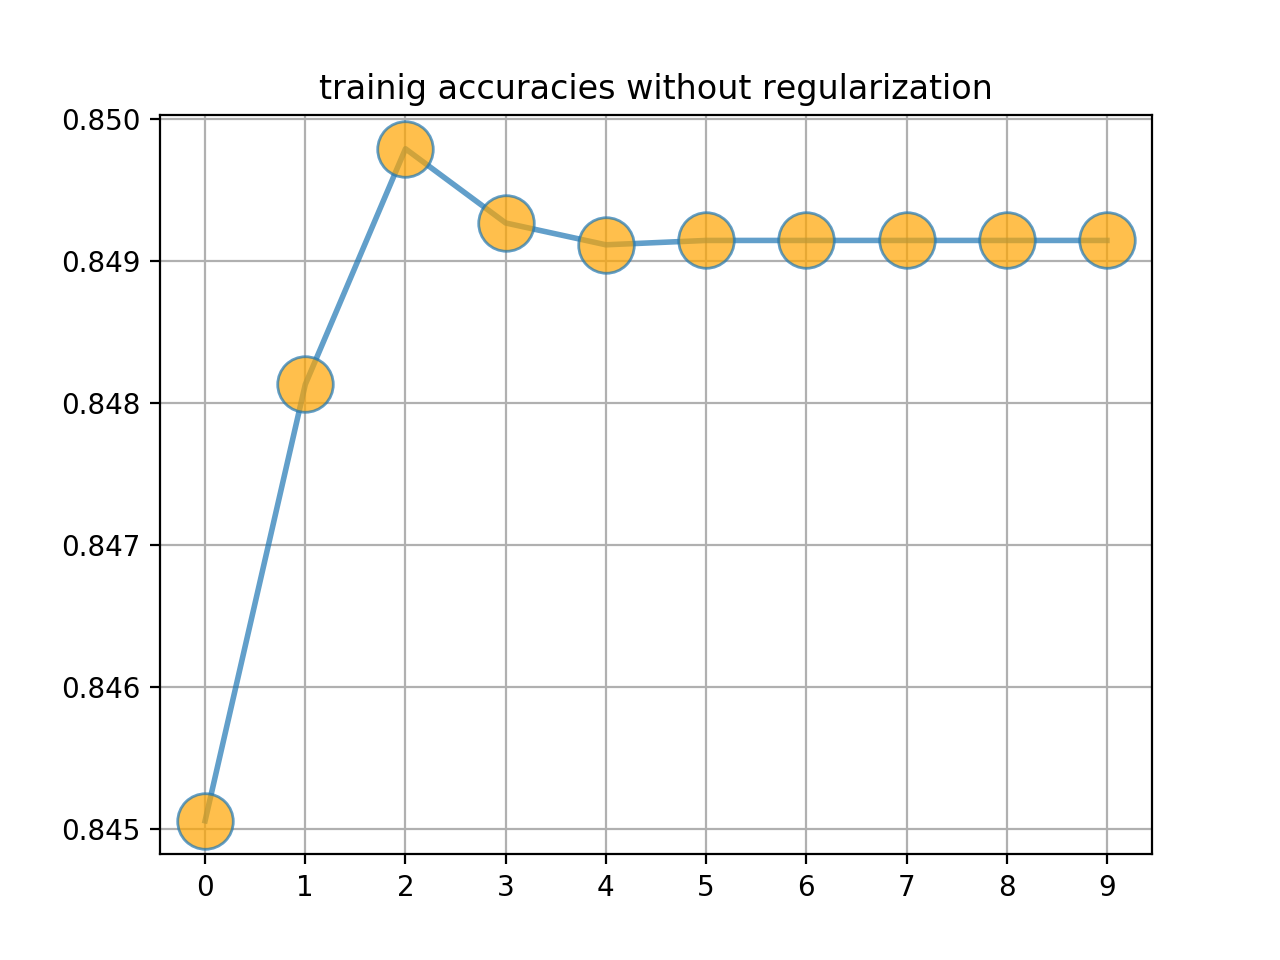
\includegraphics[scale=0.47]{t0.png}
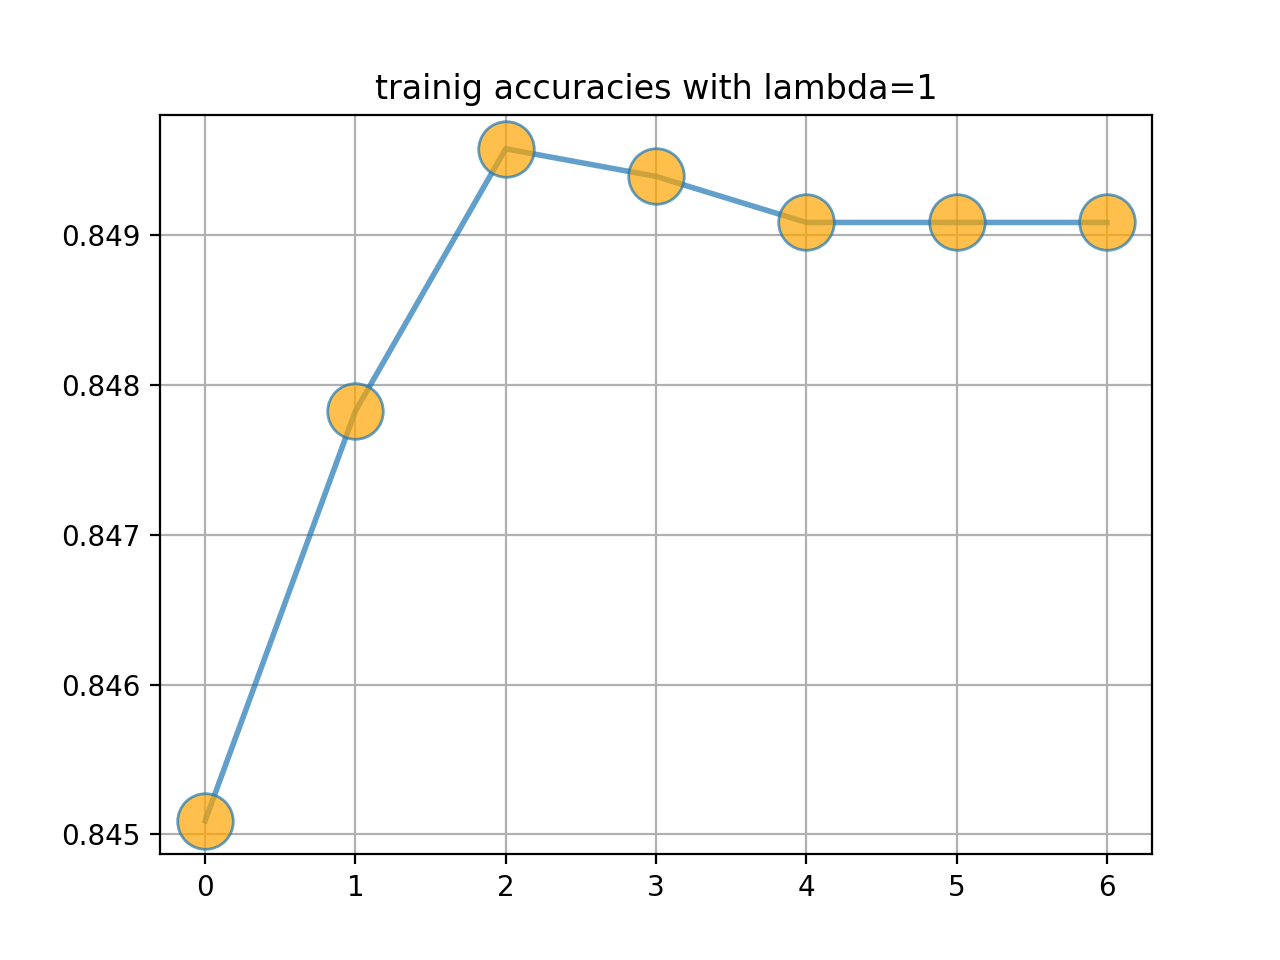
\includegraphics[scale=0.47]{t1.png}
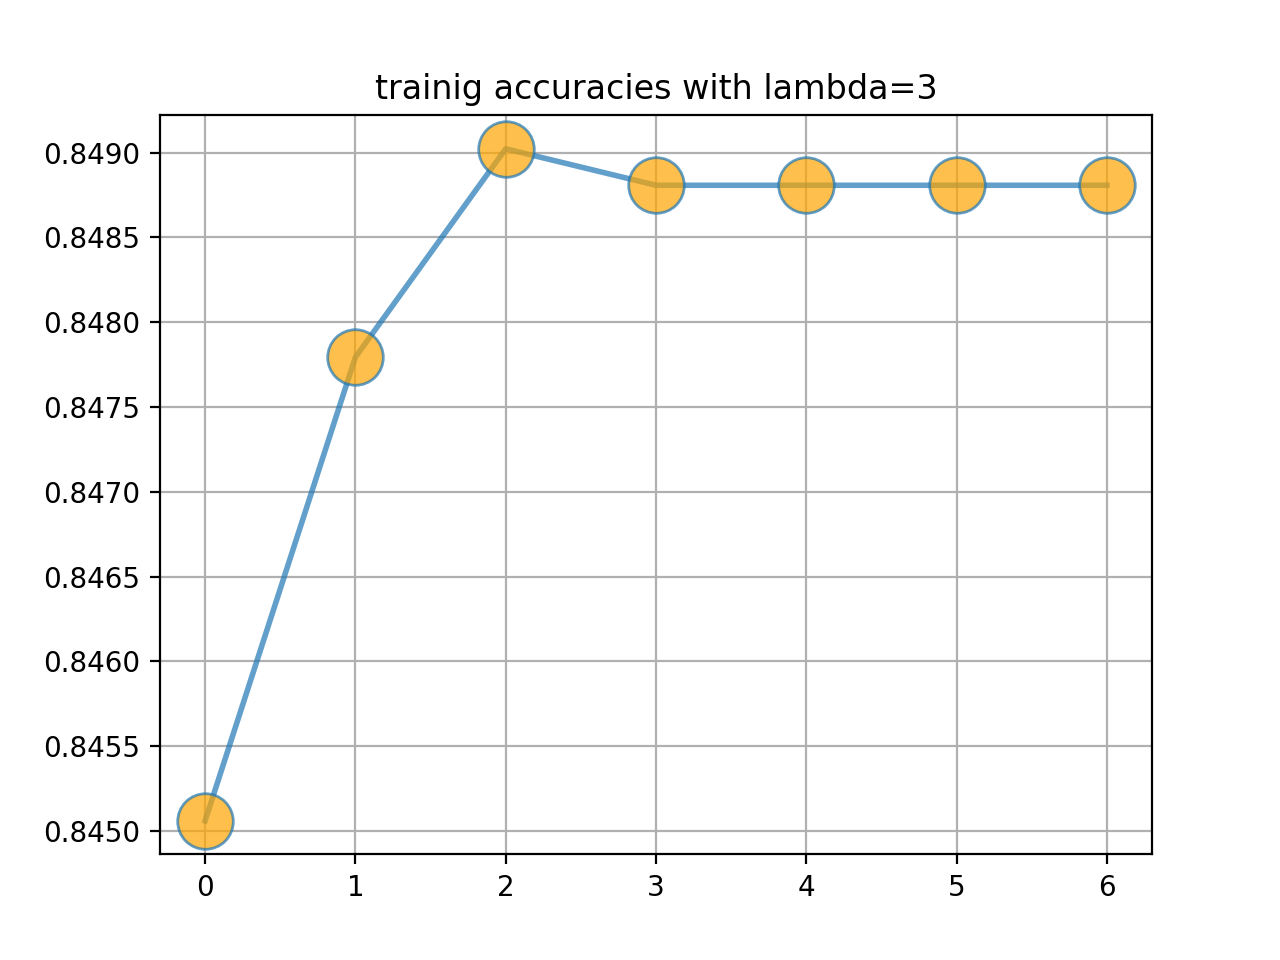
\includegraphics[scale=0.47]{t3.png}
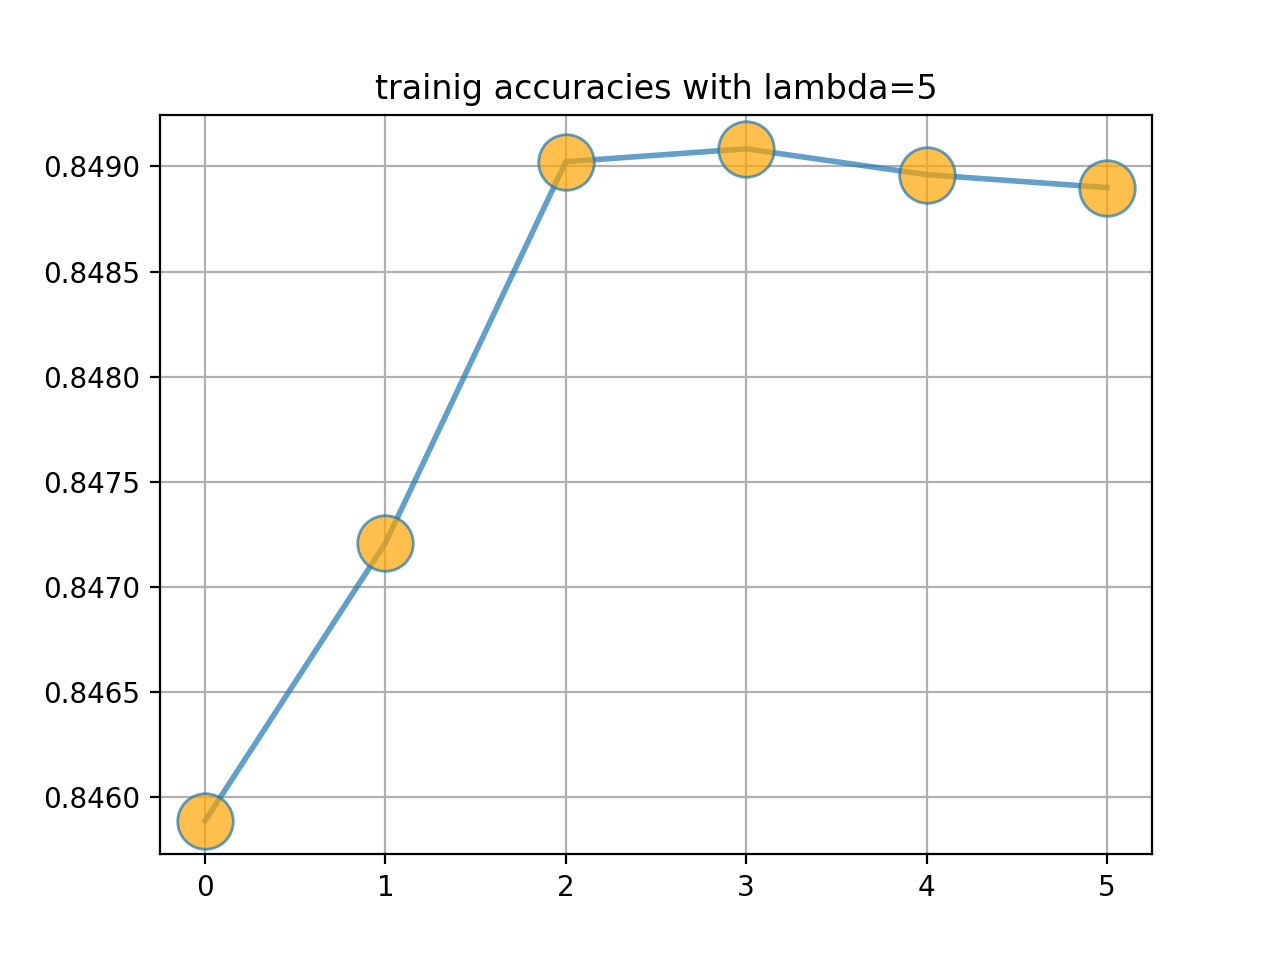
\includegraphics[scale=0.47]{t5.png}
\end{figure}

As we can find, the update iteration of $\omega$ gets smaller when $\lambda$ gets larger. 
\par
Then we test the weights on the test data, and adjust the value of $\lambda$ to see the optimal accuracy, as shown in the next page.
\newpage
The testing accuracies with different values of lambda are shown below:
\begin{figure}[ht]
\centering
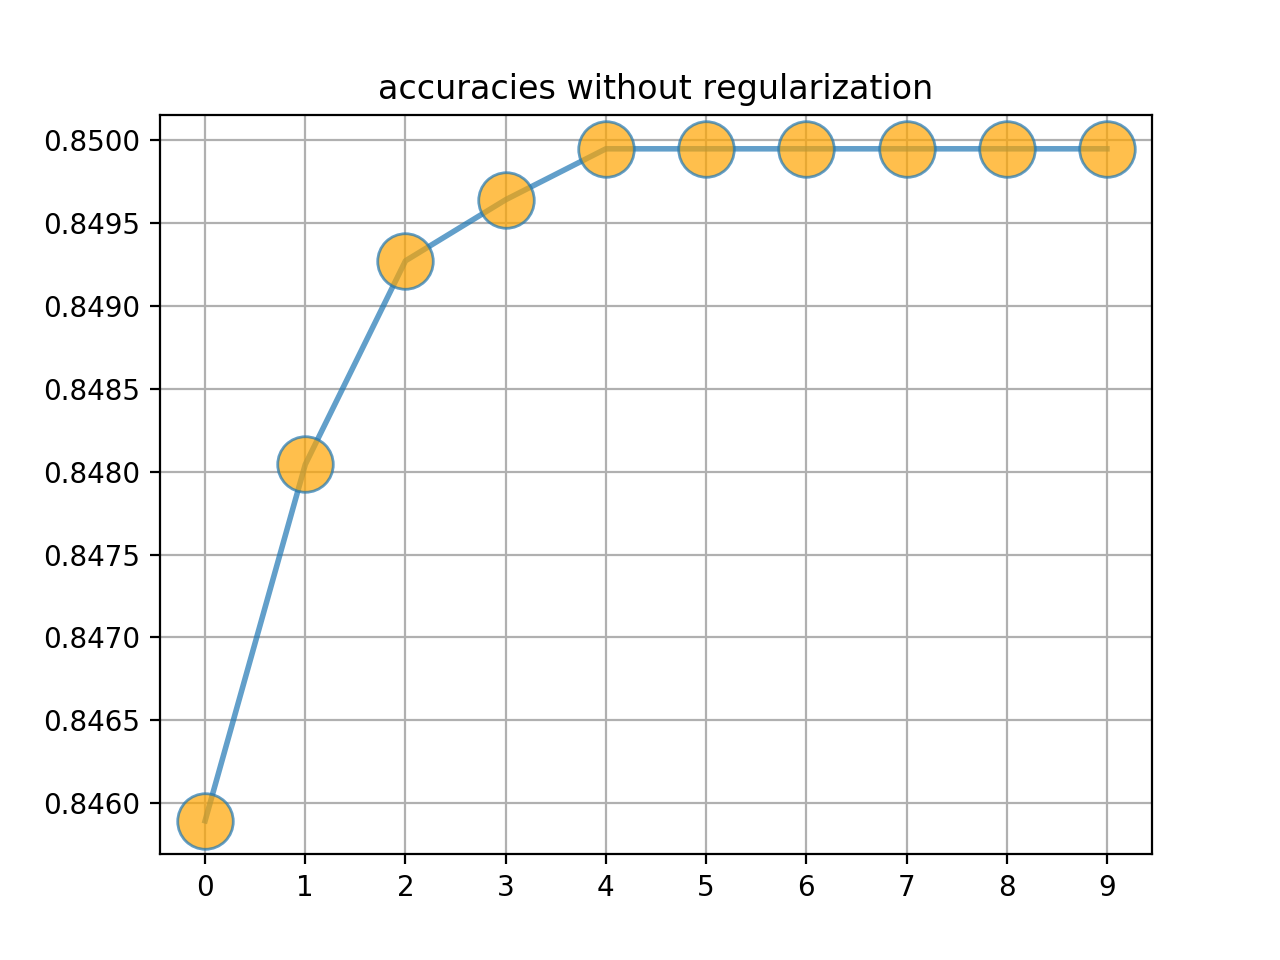
\includegraphics[scale=0.47]{1.png}
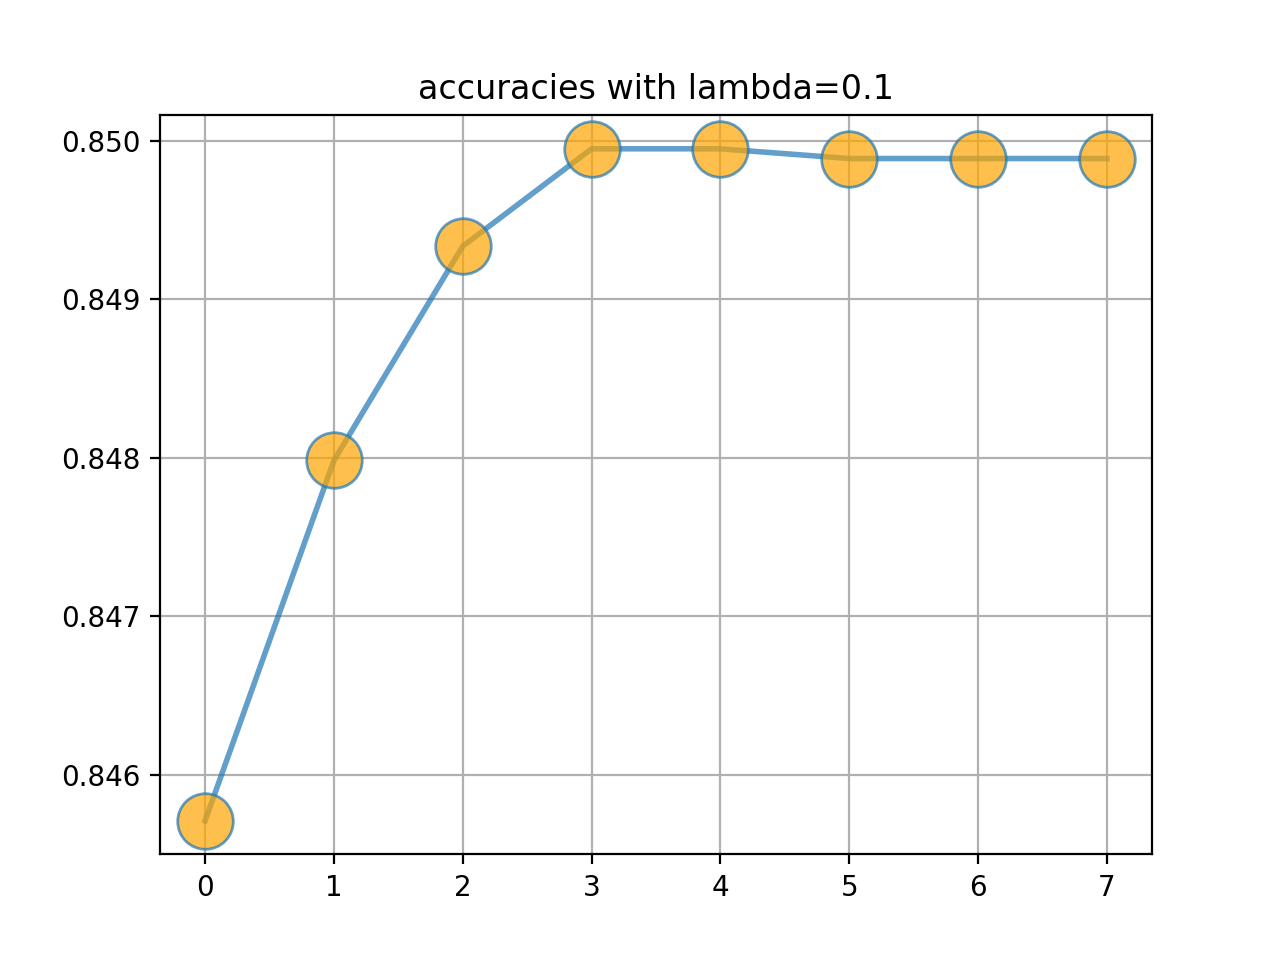
\includegraphics[scale=0.47]{2.png}
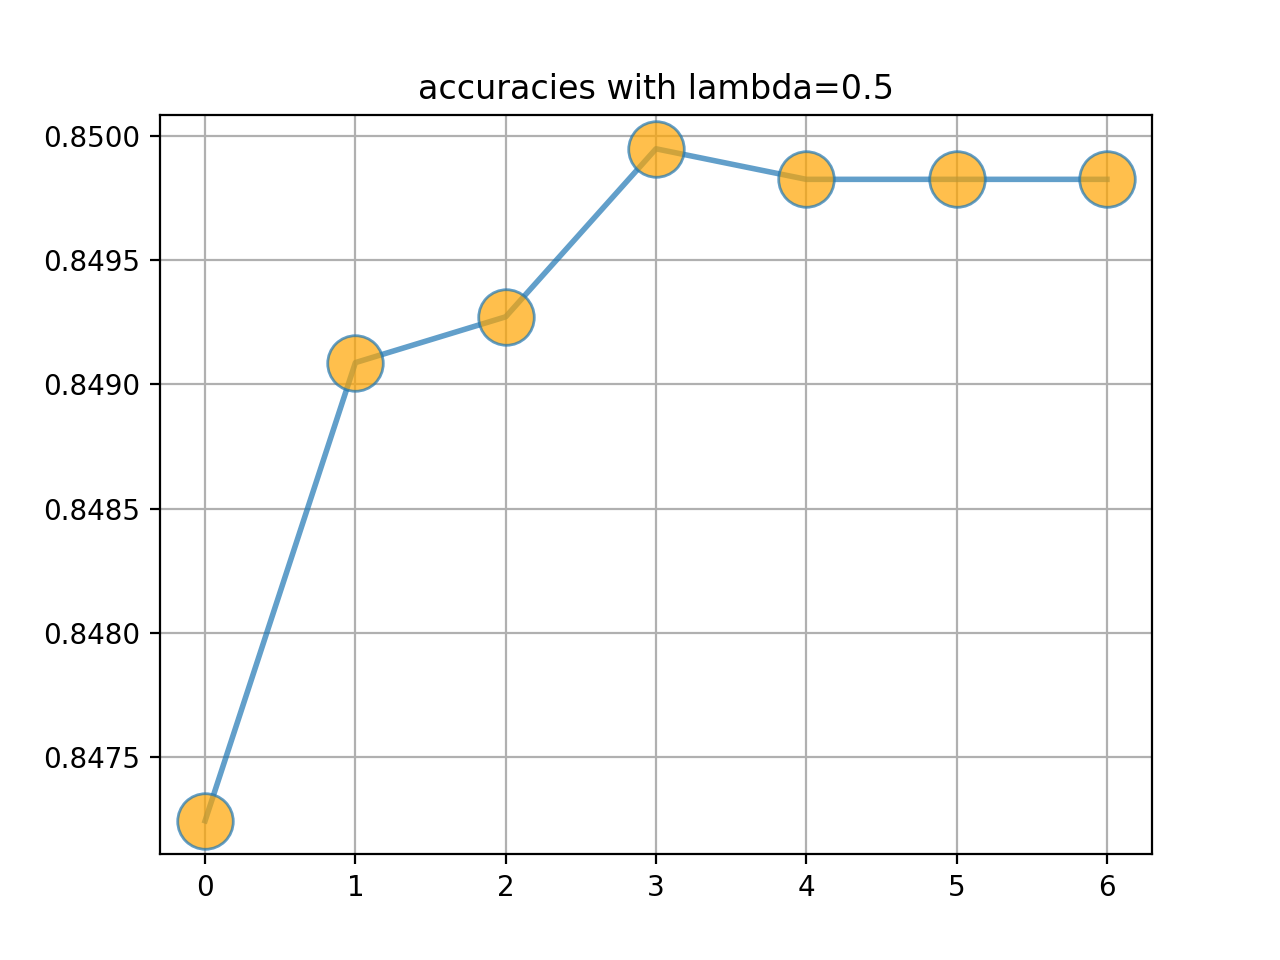
\includegraphics[scale=0.47]{3.png}
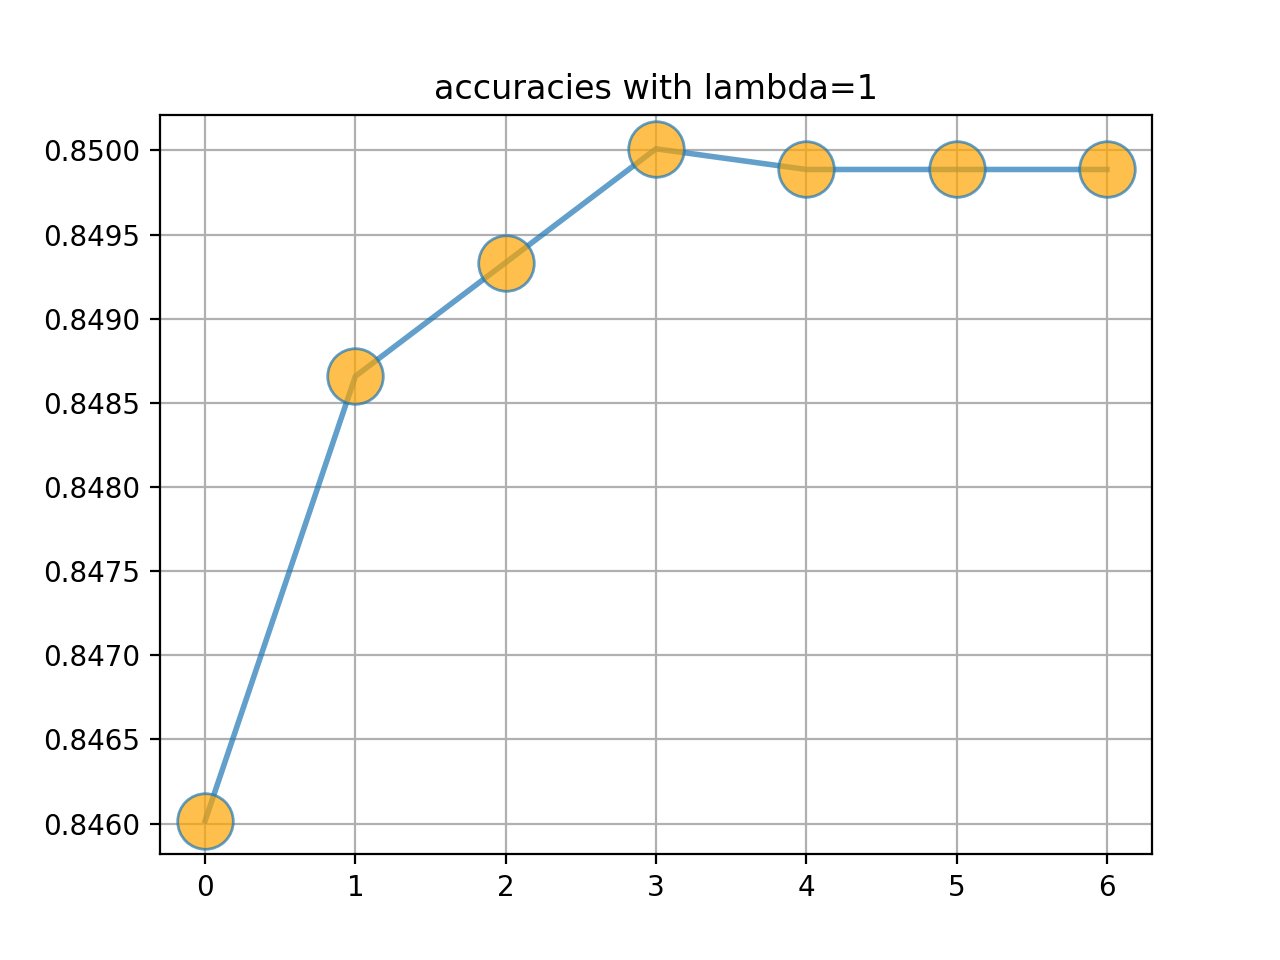
\includegraphics[scale=0.47]{4.png}
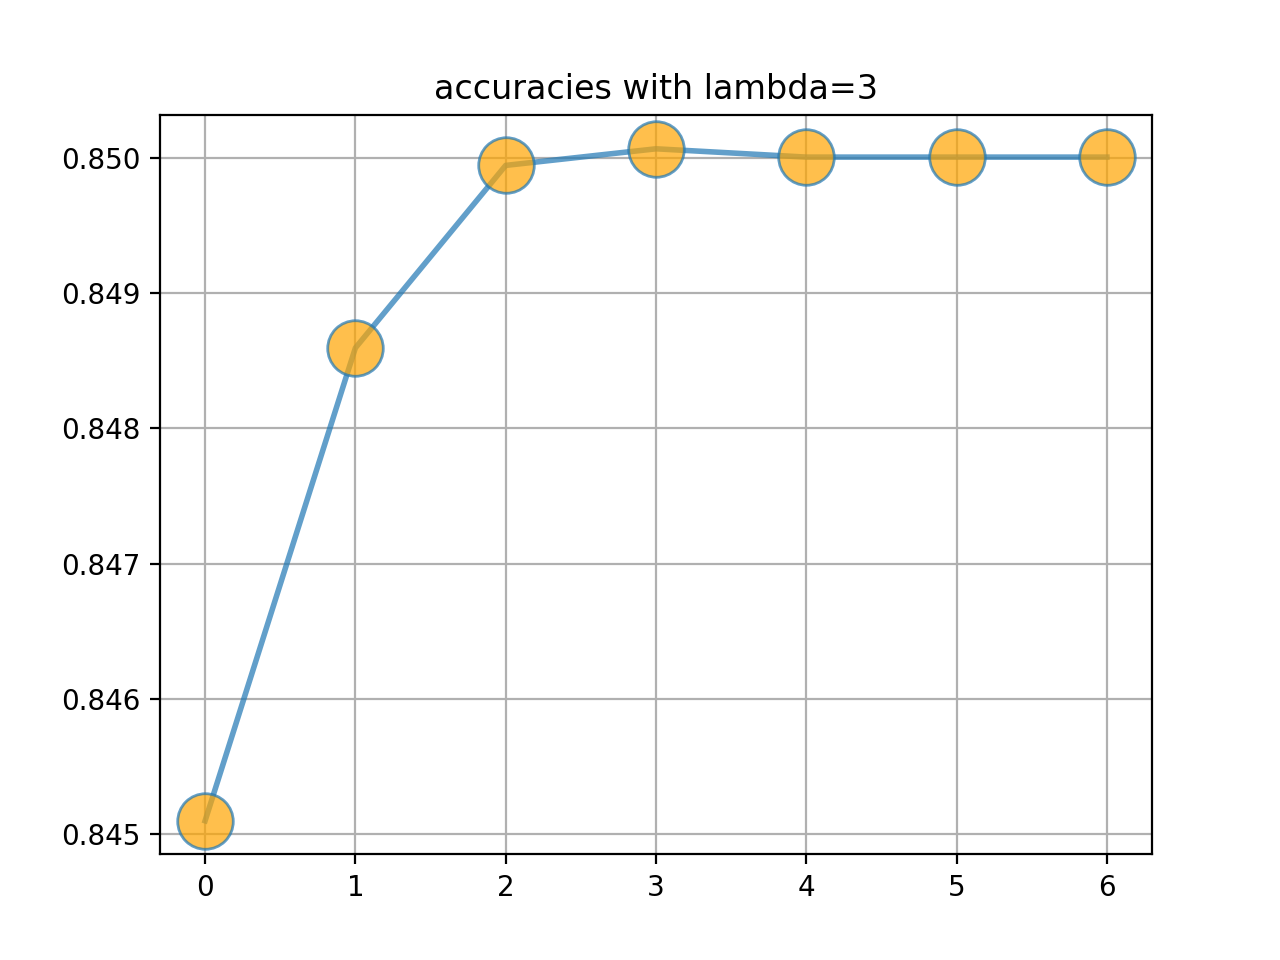
\includegraphics[scale=0.47]{5.png}
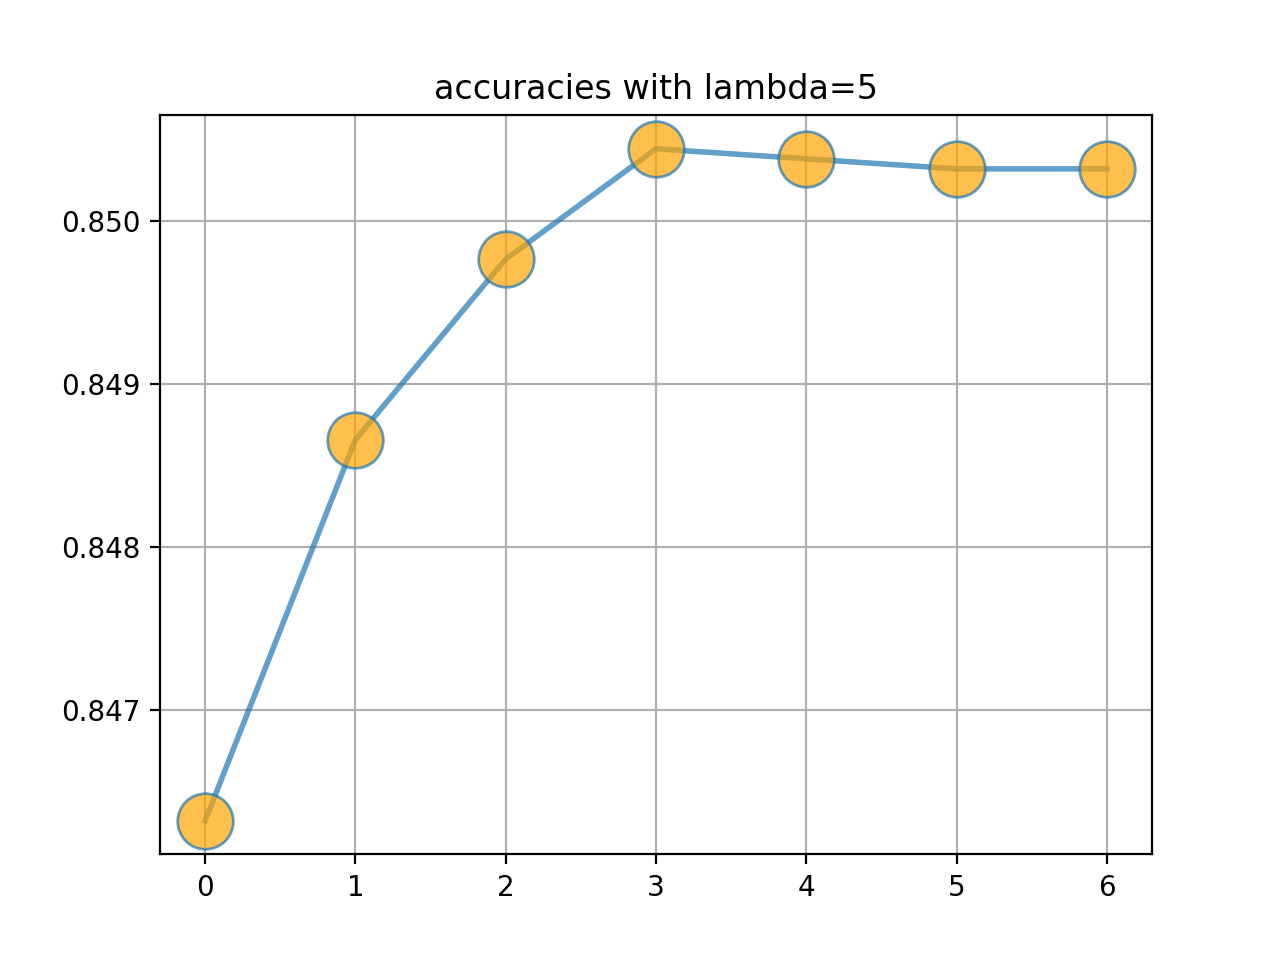
\includegraphics[scale=0.47]{6.png}
\end{figure}

\newpage
Therefore when $\lambda\in[30,80]$, the testing accuracy seems to reach the optimal value $85.1\%$. 
\begin{figure}[ht]
\centering
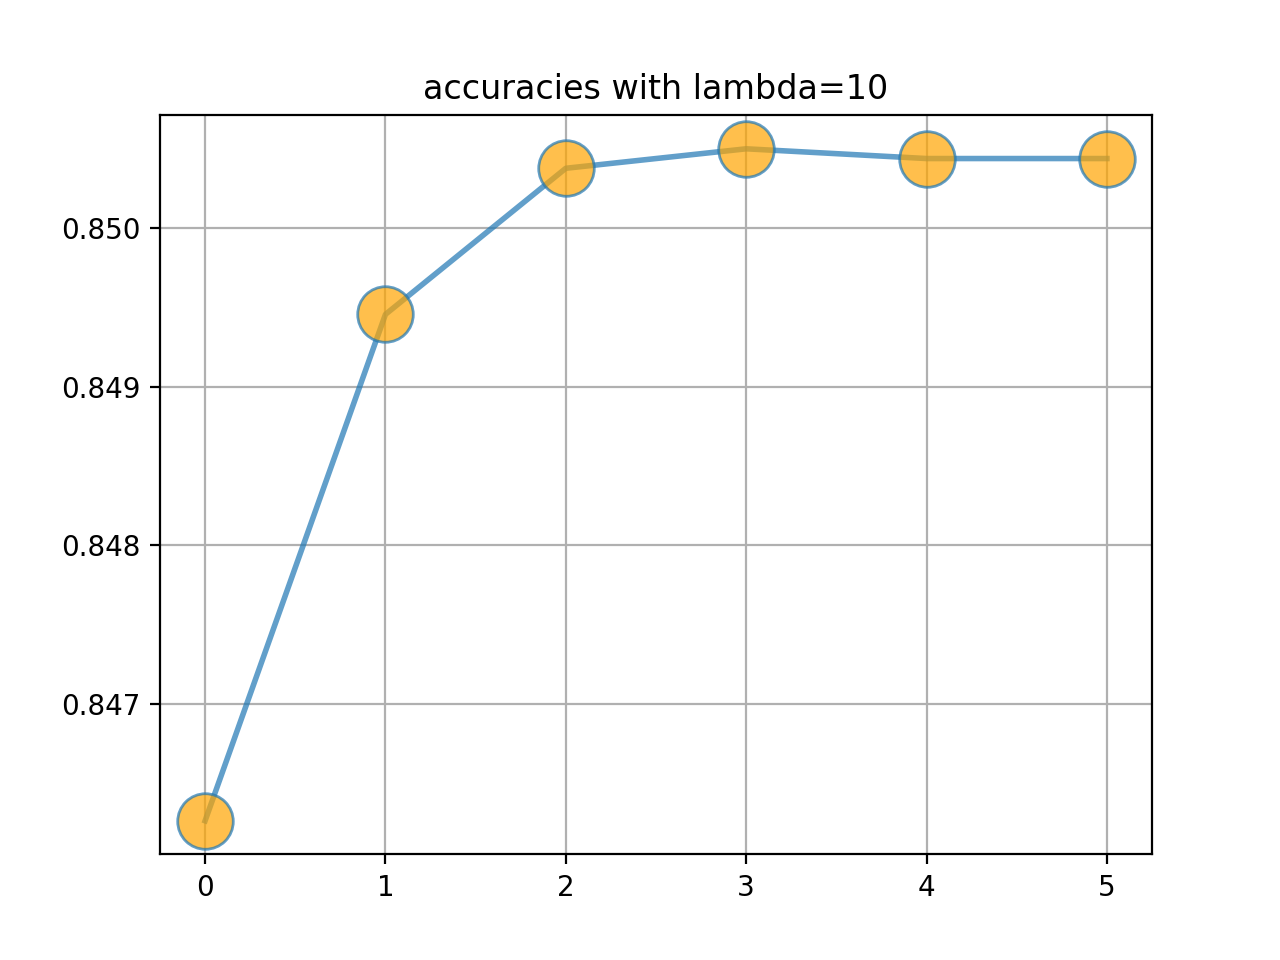
\includegraphics[scale=0.47]{7.png}
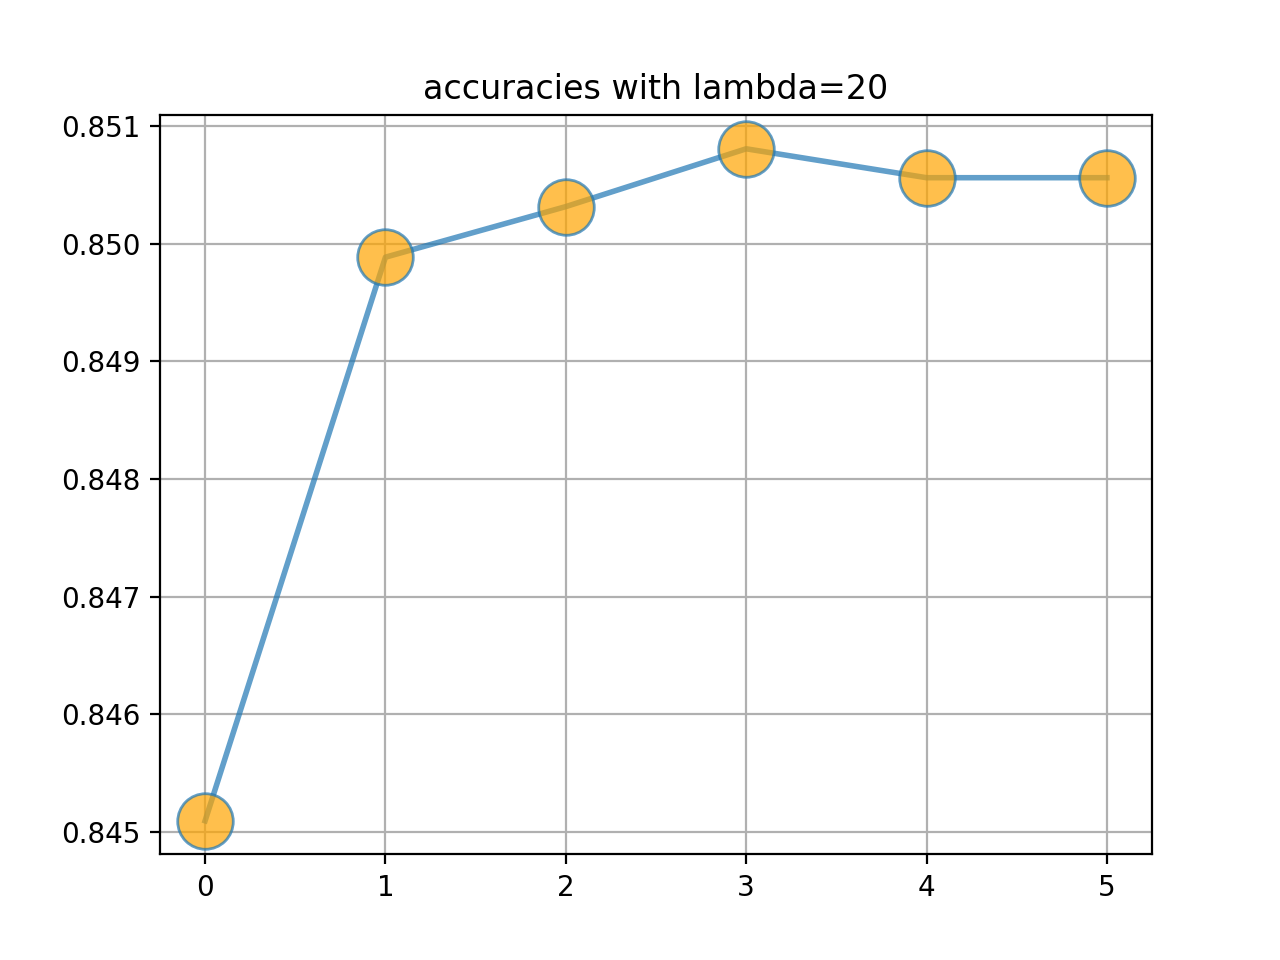
\includegraphics[scale=0.47]{8.png}
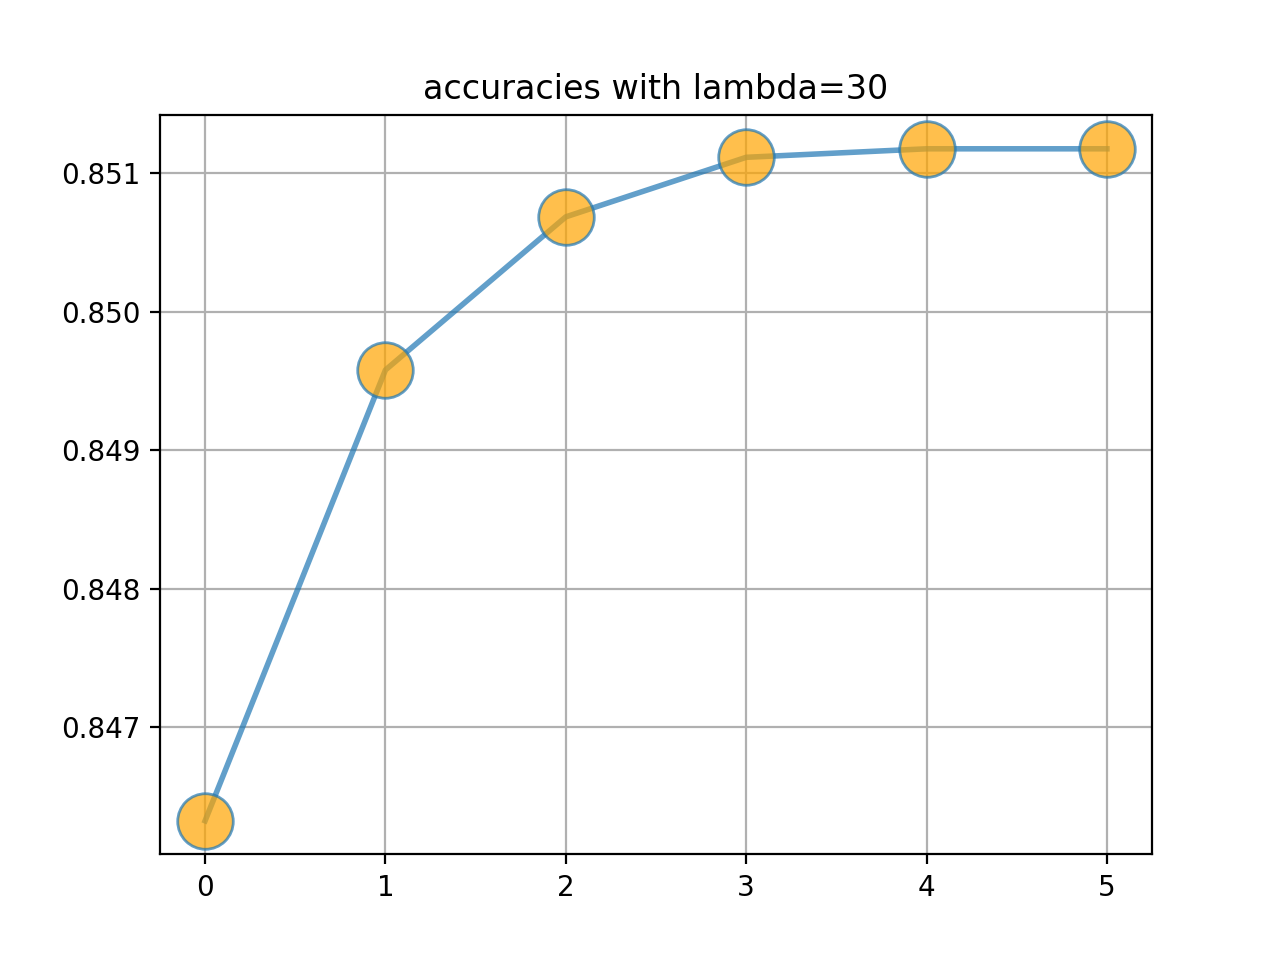
\includegraphics[scale=0.47]{9.png}
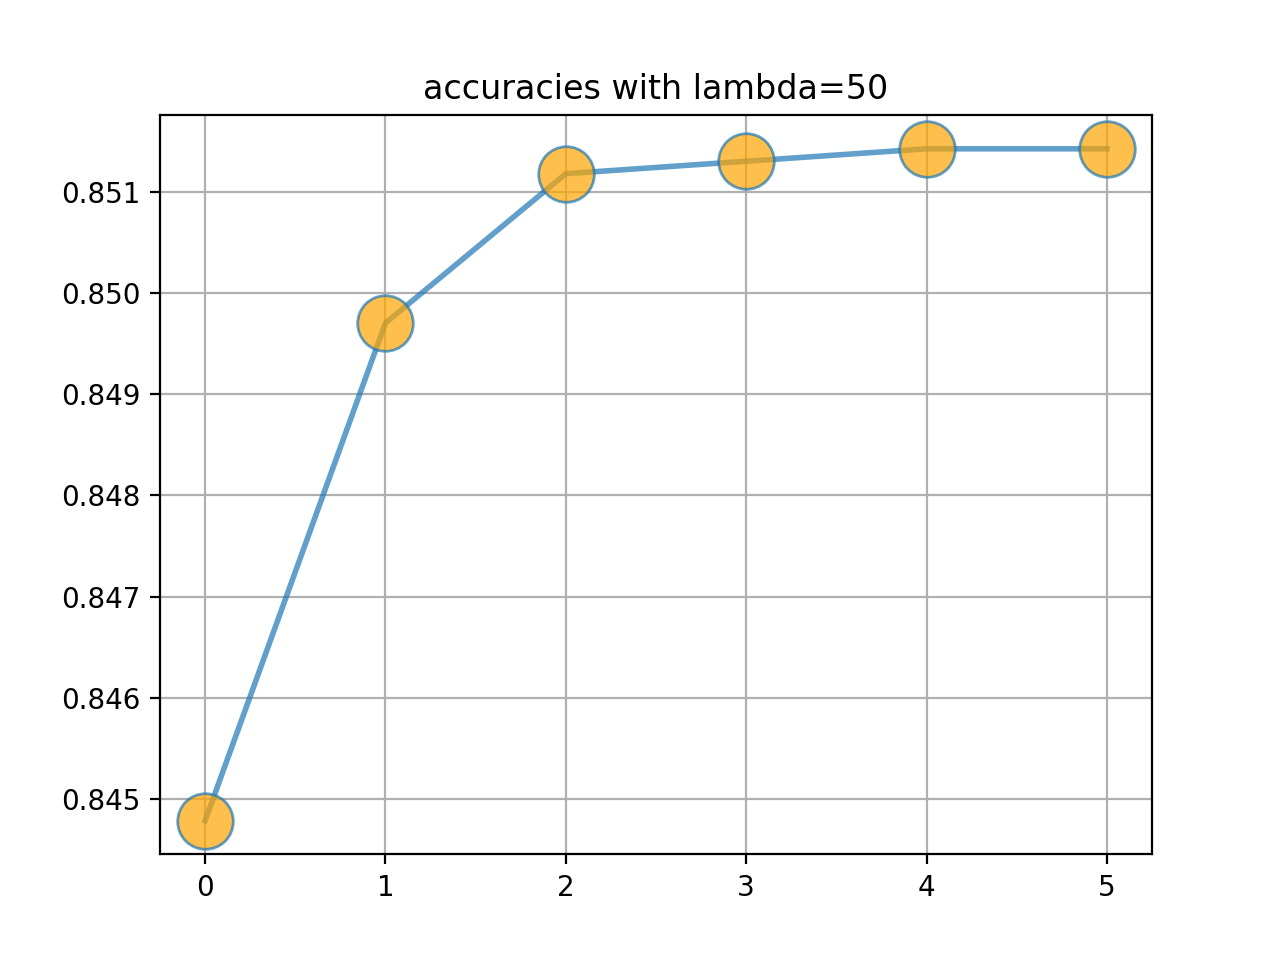
\includegraphics[scale=0.47]{10.png}
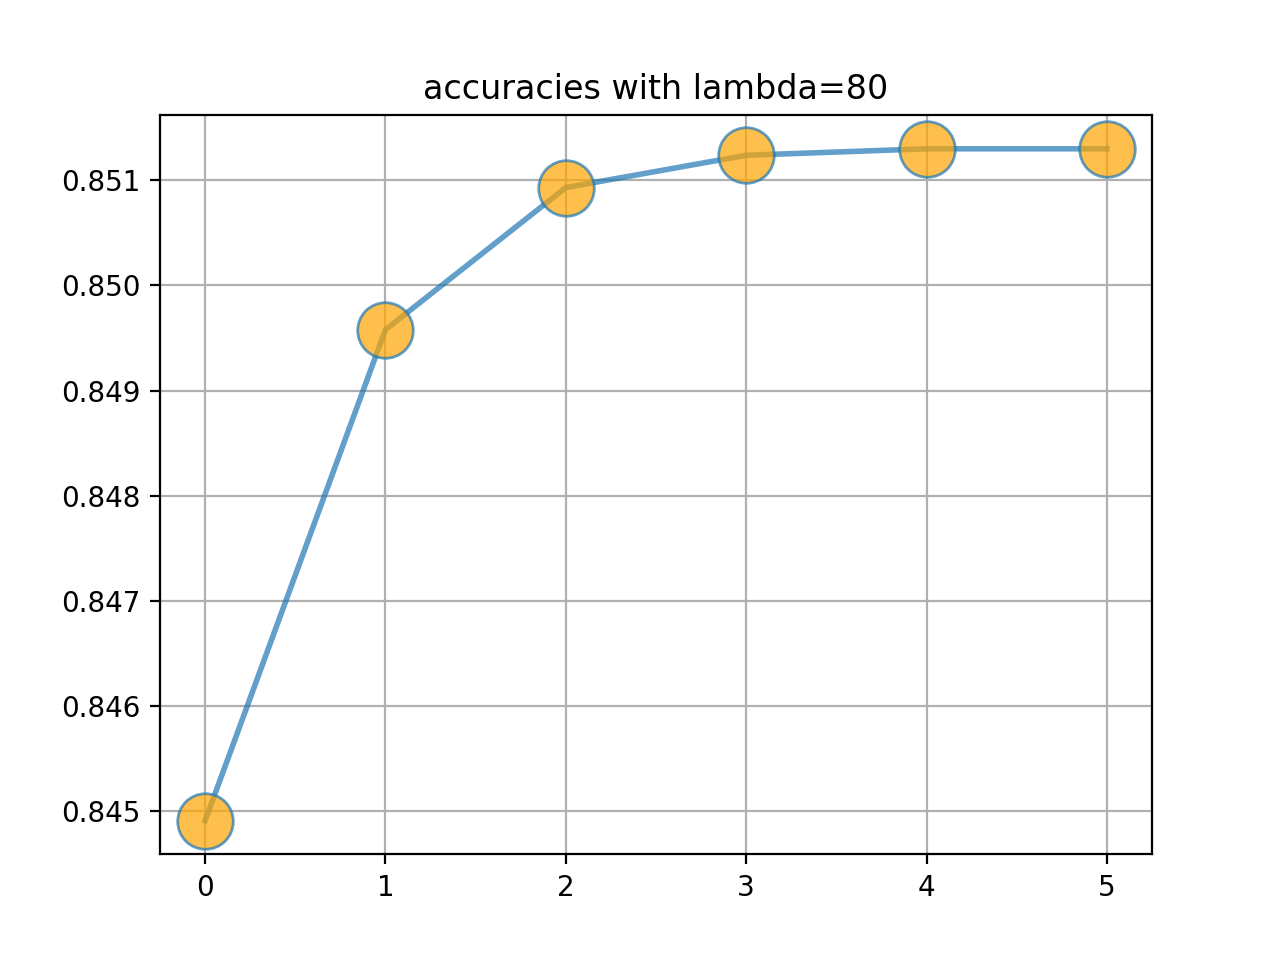
\includegraphics[scale=0.47]{11.png}
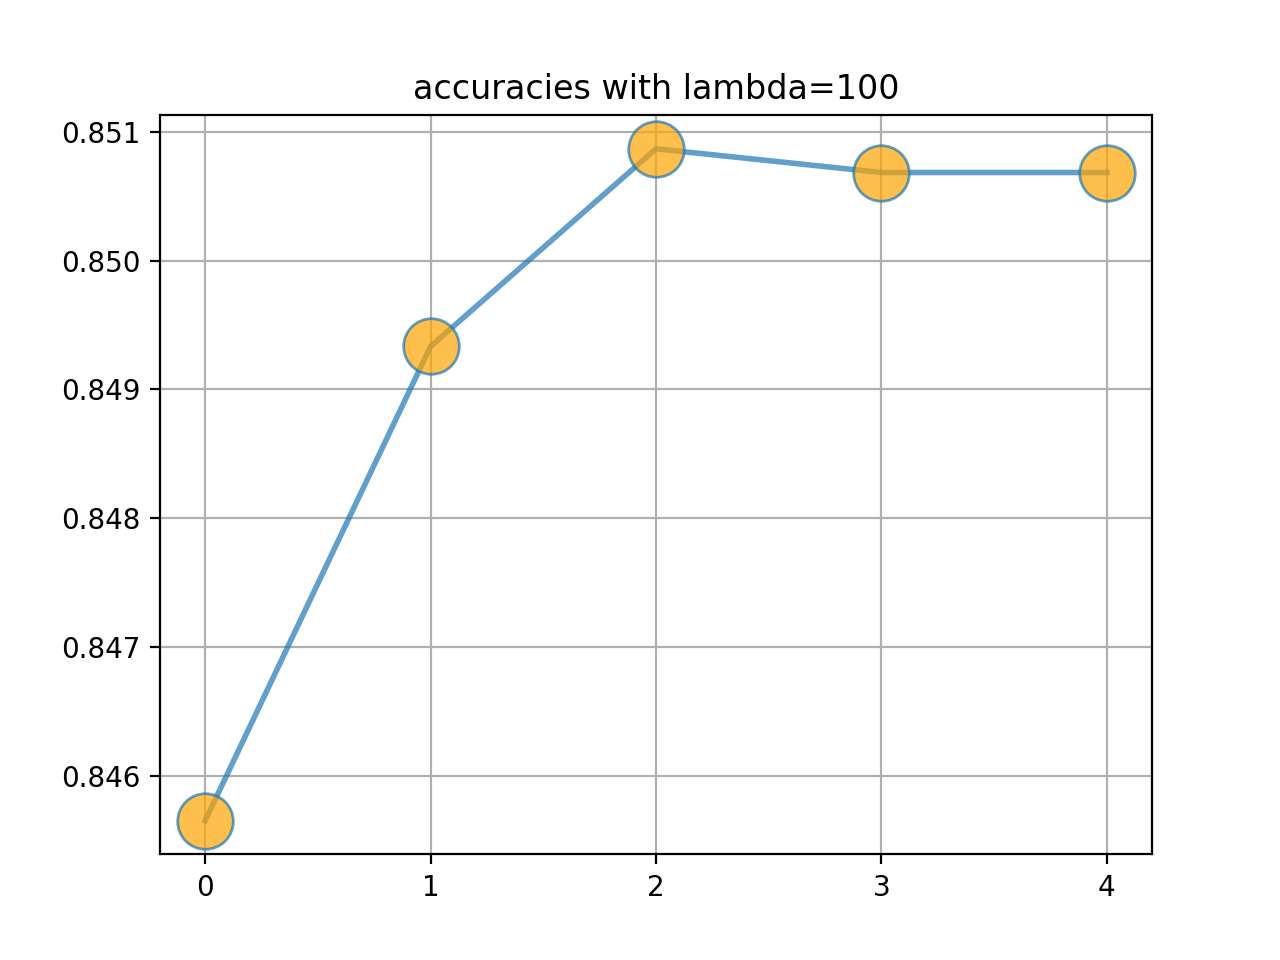
\includegraphics[scale=0.47]{12.png}
\end{figure}


\end{document}